\documentclass{mai_book}

\defaultfontfeatures{Mapping=tex-text}
\setdefaultlanguage{russian}

\usepackage{fancyhdr} %загрузим пакет
\usepackage{amsfonts}
\pagestyle{fancy}% применим колонтитул
\usepackage{color}

%\usepackage{colortbl}
%\usepackage{tikz}
%\graphicspath{{noiseimages/}}
\fancyhead{} %очистим хидер на всякий случайMAI
%\usepackage[dvips]{graphicx}
%\fancyhead[LO]{текст} 
\setcounter{page} {706}
\fancyhead[LE, RO]{\thepage}
% \newtop{ЗАГОЛОВОК}  юзать чтобы вручную поменть заголовок вверху страници
\begin{document}
	\fancyhead[RE, LO]{706}
	\fancyhead[LE, RO]{Литература}
\noindent [136] Nogu\`{e}s R . {\itshape Theoreme de Fermat. Son histoire,} Vuibert, Paris, 1932.
\newline
[137] Nussbaumer H.J. {\itshape Fast Fourier transform and convolution algorithms,} Sprin\\ger-Verlag, 1982. [Русский перевод: Нуссбаумер Г. Быстрое преобразование Фурье и алгоритмы вычисления свертки. — М.: Радио и связь, 1985.]
\newline
[138] Oesterl\'{e} J. “Nombres de classes des corps quadratiques imaginaires”, S\'{e}minaire N. Bourbaki, n° 631, 06 1984.
\newline
\noindent[139] Oesterl\'{e} J. “Nouvelles approches du theoreme de Fermat”, {\itshape S\'{e}minaire N. Bourbaki,} n° 694, 02 1988.
\newline
[140] Ozello P. {\itshape Calcul exact des formes de Jordan et de Frobenius d’une matrice,} These de $3^{e}$-cycle Univ. Grenoble, 1987.
\newline
\noindent [141] Pascaud J.L. “Calcul des coefficients de Bezout dans l’anneau des entiers de $\mathbb{Q}(\sqrt{-19})$”, Janvier. 1988.
\newline
[142] Perlis A. J. “Epigrams on programming”, {\itshape Communication prive\'{e}, ACM Sigplan Notices,} 1975.
\newline
\noindent [143] Perrin D. “Cours d’alg\'{e}bre”, Publications de l’E.N.S. de Jeunes Filles, n° 18, 1982.
\newline
\noindent [144] Pohst M. {\itshape Algorithmic methods in algebra and number theory,} Academic Press, 1987.
\newline
[145] Poitou G. “Solution du probl\'{e}me du dixi\'{e}me discriminant (d’apr\'{e}s Stark)”, S\'{e}minaire N. Bourbaki, n° 335, 11 1967.
\newline
[146] Pollard J.M.  “The Fast Fourier Transform in a Finite Field”, {\itshape Math. Comp.}, vol. 25, n° 114, 1971, pp. 365-374. [Имеетсяперевод: В кн. Макклеллан Дж. Х., Рейдер Ч.М. {\itshape Применение теории чисел в цифровой обработке сигналов.} — М.: Радио и связь, 1983, с. 147-155.]
\newline
[147]  Pollard J.M. “Monte Carlo methods for index computation mod {\itshape p}”, {\itshape Math. Comp}., vol. 32, n° 143, 1978, pp. 918-924.
\newline
[148] Pomerance C., Selfridge J.L., Wagstaff S.S. “The pseudoprimes to $25.10^{9}$”, {\itshape Math. Comp}., vol. 35, n° 151, 1980, pp. 1003-1026.
\newline
[149] Popper K. R . {\itshape La Iogique de la d\'{e}couverte scientilique, traduit par} N. Thyssen-Rutten et P. Devaux, Payot.
\newline
[150] Rabin M.O. “Probalistic algorithm for testing primality”, {\itshape Journal of Number Theory}, vol. 12, 1980, pp. 128-138.
\newline
[151] Rabin M. O. “Digitalized signatures and public-key functions as in­ tractable as factorization”, Cambridge, MA, 1979.
\newline
[152] Rader C. M. “Discrete Fourier transform when the number of data sam­ ples is prime”, Proc. IEEE, Mass. Inst, of Tech., vol. 5, n° 6, 1968, pp. 1107-1108. [Имеется перевод: в сб. [146].]
\newline
[153] Ribenboim Р . {\itshape 13 Lectures on Fermat’s last theorem}, Springer-Verlag, 1979.

\newpage
\fancyhead[RE, LO]{707}
\fancyhead[LE, RO]{Литература}
%\fancyhead[LE]{Литература}
\noindent
[154] Ribenboim Р. {\itshape The Book of Prime Number Records}, Springer-Verlag, 1980.
\newline
[155] Riesel H. {\itshape Prime Numbers and Computers Methods for Factorization}, Birka\"{u}ser Boston, Inc., 1985.
\newline
[156] Rivest R. L., Shamir A., Adleman L. “A method for obtaining dig­ ital signat\\ures and public-key cryptosystems”, {\itshape Comm. ACM}, vol. 21, n° 2, 1978, pp. 120-126.
\newline
[157] ROSE D. J. “Matrix Identities of the Feist Fourier Transform”, {\itshape Linear Al­ gebra and Appl}., vol. 29, 1980, pp. 423-443.
\newline
{scshape [158] Rousseau G. “Exterior algebras and the quadratic reciprocity law”, {\itshape L’enseignement Math\'{e}matique}, vol. 36, 1990, pp. 303-308.
\newline
[159] Samuel P. “About Euclidean Rings”, {\itshape J. Algebra}, vol. 19, 1971.
\newline
[160] Samuel P. {\itshape Th\'{e}orie alg\'{e}brique des nombres}, Hermann, 1967.
\newline
[161] Schmid A. F. {\itshape Une philosophic de savant, Henri Poincar\'{e} et la logique math\'{e}matique}, Francois Maspero, 1978.
\newline
[162] Sch\"{o}nhage A., Strassen V. “Schnelle Multiplikation Grossen Zahlen”, {\itshape Computing}, vol. 7, 1971, pp. 281-292. [Русский перевод: В сб. Кибернетичес- \\кий сборник. Новая серия. Вып. 10. — М.: Мир, 1973.]
\newline
[163] Shamir A. “A polynomial time algorithm for breaking the basic Merkle-Hellman cryptosystem”, {\itshape Proc. 23rd Annual Symp. Found. Comput. Sci}., 1982, pp. 145-152.
\newline
[164] Shamir A. “How to share a secret”, {\itshape Comm. ACM}, vol. 22, n° 11, 1979.
\newline
[165] Sims C. G. {\itshape Algebra, A Comput. Approach}, John Wiley {\textit \&} Sons, 1984.
\newline
[166] Stark H. M. “A complete determination of the complex quadratic fields of class-number one”, {\itshape Michigan Math. J.}, vol. 14, 1967, pp. 1-27.
\newline
[167] Steild G., Tasche M. “Index Transforms for Multidimensional DFT’s and Con”, vol. 56, 1989, pp. 513-528.
\newline
[168] Tanenbaum A. {\itshape Architecture des ordinateurs}, Inter\'{e}ditions, 1986.
\newline
[169] Terras R. “A stopping time problem on the positive integers”, {\itshape Acta arithme\\tica}, vol. 30, 1987, pp. 241-252.
\newline
[170] Thomson K. “Reflections on trusting trust”, {\itshape Comm. ACM}., vol. 27, n° 8, 1984, pp. 761-763.
\newline
[171] Vaser\v{s}tein L. N. “On the group $SL_{2}$ over Dedekind ring of arithmetic type”, {\itshape Math. USSR. Sbornick}, vol. 18, n° 2, 1972, pp. 321-332.
\newline
[172] Wagon S. “Editor’s Comer : The Euclidean Algorithm Strikes Again”, {\itshape Amer. Math. Monthly}, vol. 97, n° 2, 1980, pp. 125-129.
\newline
[173] Wagstaff S. S. {\itshape Divisors ofMersenne numbers}, 1983.
\newline
[174] Washington C. L. {\itshape Introd. to Cyclotomic Fields}, Springer-Verlag, 1980.
\newline
[175] Weinberger P. J. “On euclidean rings of algebraic integers”, {\itshape Proc. Amer. Math. Soc. Symp. Pure Mathematics, Math. Comp}., vol. 40, n° 24. 1973, pp. 321-332.
\newline
\newline
\noindent{\footnotesize 45*}

\newpage
%\setcounter{page}{708}
%\newtop{Литература}
\fancyhead[RE, LO]{708}
\fancyhead[LE, RO]{Литература}
\noindent
[176] Winograd S. “On the number of multiplications necessary to compute certain functions”, {\itshape Comm. Pure Appl. Math}., vol. 23, 1970, pp. 165-179.
\newline
[177] Winograd S. “On Multiplication of Polynomials Modulo a Polynomial”, {\itshape R.C. 6791, IBM Research}, 1977.
\newline
[178] Winograd S. “On Computing the Discrete Fourier Transform”, {\itshape Math. Comp}., vol. 32, n° 141, 1978, pp. 175-199. [Имеется перевод: в сб. [146].]
\newline
[179] Winograd S. “Some bilinear forms whose multiplicative complexity depends on the field of constants”, {\itshape Math. Syst. Theory}, vol. 10, 1977, pp. 169-180.
\newline
[180] Winograd S. “On the Multiplicative Complexity of the Discrete Fourier Transform”, {\itshape Advances in Mathematics}, vol. 32, 1979, pp. 83-117.
\newline
[181] Wirth N. {\itshape Algorithms + Data Structures = Programs}, Prentice Hall, 1976. [Русский перевод: Вирт H. {\itshape Алгоритмы + структуры данных = программы}. — М.: Мир, 1985.] \newline
[182] Wirth N. {\itshape Introduction \`{a} la programmation syst\'{e}matique}, Masson, 1977. \newline
[183] Yates F. “The Design and Analysis of Factorial Experiments”, {\itshape Imperial Bureau of Soil Sciences}, 1937.
\newline
[184] Young J., Buell D. “The twentieth fermat number is composite”, {\itshape Math. Comp}., vol. 50, n° 181, 1988, pp. 261-263. \newline

\begin{center}

{\large \textbf{Литература, добавленная к изданию}}

\end{center}

\noindent[185] Биркгоф Г., Барти Т. {\itshape Современная прикладная алгебра}. — М.: Мир, 1976. \newline
[186]
Джехани Н. Язык Ада. — М.: Мир, 1988.
\newline
[187] Калужнин Л.А. {\itshape Введение в общую алгебру}. — М.: Наука, 1973. \newline
[188] Кострикин А. И. {\itshape Введение в алгебру}. — М.: Наука, 1977.\newline
[189] Лидл Р., Пильц Г. {\itshape Прикладная абстрактная алгебра}. Учебн. пособие, Екатеринбург: Изд-во Урал, ун-та, 1996. \newline
[190] Перминов О. Н. {\itshape Введение в язык программирования Ада}. — М.: Ра­ дио и связь, 1991.\newline
[191] Прасолов В. В., Соловьев Ю. П. {\itshape Эллиптические функции и алгебраичес\\кие уравнения}. — М.: Факториал, 1997, 288 с.
\newline
[192] Gill A. {\itshape Applied Algebra for the Computer Science}, Prentice-Hall, Engle­ wood Cliffs, N.F., 1976.
\newline
[193] Ribenboim P. {\itshape Fermat’s Last Theorem}. For Amateurs, Springer-Verlag, 1999, 407 p. \newline
[194] Singh S. {\itshape Fermat’s Enigma: The Epic Quest to Solve the World’s Greatest Mathematical Problem}, Walker and Company, N.Y., 1997, 288 p.
\newline
[195] Wiles A. {\itshape Modular elliptic curves and Fermat’s Last Theorem}, Ann. Math. 141, 1995, c. 443-551.

\newpage
\fancyhead{}
\thispagestyle{empty}
\fancyhead[RE]{Алфавитный указатель} 
\hfill \break
\hfill \break
\hfill \break
\begin{center}
{\Large\textbf{Алфавитный указатель}} \\
\hfill \break
Номера страниц, относящиеся к упражнениям, выделены курсивом.
\end{center}


\begin{tabular}{llcc}
	SL$_{2}$($\mathbb{Z}$), {\itshape 373} & Возведение в степень, \emph{136} \\
	$\mathbb{Q}(\sqrt{19})$, {\itshape 268} & -- дихотомическое, 32, 33, 37, \\
	emph{n}!, 64, {\itshape 247} & \emph{111} \\
	 2-группа, 493, 497 & -- сложность, {\itshape 102} \\
	& Вычет квадратичный, 185, \emph{249}, \\ 
	mod (оператор), 194, 197 & \emph{299}, 479, 485, {\itshape 526}, {\itshape 527, 555}\\ 
	
	& Гаусс, 57, 233 \\ 
	rem (оператор), 197 & -- лемма, 232\\ 
	& -- свойство, 188, 191\\
Алгебра Берлекэмпа, {\itshape 541} & -- сумма, 483\\ 
	-- тензорное произведение, 656 & -- теорема, 233 \\ 
	- циклической свертки, 593 & - целые числа, 182, 195,{\itshape  248} \\ 
	Аннулятор & Горнера метод, 136, {\itshape 659} \\ 
	-- абелевой группы, 451 & Грея код, {\itshape 106, 108} \\ 
	-- модуля, 325, 366 & Группа абелева \\ 
Аппроксимация, \emph{245} & -- \emph{p}-примарная, 452 \\ 
	Арифметика & -- конечная, {\itshape 376, 380, 385, 386, } \\ 
	-- модулярная, 420, 425, 428, & 451, 454, \emph{526} \\ 
	-- основная теорема, 179 & -- конечная двойственная, \emph{668-} \\ 
		-- повышеной точности, \emph{115, 116,} & \emph{670} \\ 
 434 & - конечного типа (структурная \\ 
	 & теорема), 367 \\ 
Безу коэффициенты, 229, 230, \emph{257,}	& Группа обратимых элементов, \\
	{\itshape 259, 269, 389,} 413 & 424, 438, 463 \\ 
		-- соотношение, 179, 191, 212 & -- по модулю 2$^{r}$, 419, 460\\ 
 Берлекэмпа метод, 492, \emph{541}	& -- по модулю 3$^{r}$, 459 \\ 
	Бертрана постулат, {\itshape 99, 261} & -- по модулю \emph{n}, 442 \\
	Брента метод, 473, 516 &-- по модулю \emph{p}, 448 \\
	 & -- по модулю 125, 463\\ 
Вандермонда матрица, 586, \emph{660}	& Группа характеров, \emph{668-670} \\ 
Взаимность квадратичная, 479,	& Гуда метод, 628, 629, 650, \emph{664} \\ 

482, 484, 503, \emph{528-530}	& \\ 
Вильсона теорема, 184, \emph{247} & Дедекинда кольцо, 180 \\ 
	Виноград, 640, 650, 654, 655, \emph{671} & Деление\\ 
	Включения-исключения принцип, & - евклидово, 193, 194 \\
	\emph{110} & -- Лазара, 220 \\
\end{tabular}

	\newpage
	\fancyhead[LE, RO]{710}
	\fancyhead[RE, LO]{Алфавитный указатель} 
	
	\begin{tabular}{llcc}
	-- повышеной точности, \emph{116} & - Кольцо главных идеалов, 210, \\
	- центрированное, 195, \emph{260} & 211, {\itshape 265, 268} \\
	Дерекурсивизация, 598 & 
-- целых квадратичных чисел, \\
Диофантово уравнение, \emph{248} & \emph{252} \\
	Дирихле теорема 6/{\large$\pi^{2}$} , 221 & -- евклидово, 194, 196, 200, 201, \\
	-- теорема о прогрессиях, {\itshape 242, 526,} & 211, \emph{268} \\
	{\itshape 554, 662} & -- квазиевклидово, 218 \\
		Дробь непрерывная, \emph{242-245}, 466 & -- локальное, \emph{268} \\
			& -- нётерово, 189, 201, 231 \\
		Евклид, 177 & -- с делителями нуля, 490 \\
	-- алгоритм, 177, 193, 194, 196, 200, & -- факториальное, 181, 187, 201, \\
		205, \emph{242, 255, 256}, 260, \emph{313}, & 
211, 233, \emph{250, 265} \\
		\emph{373} & -- характеристика, \emph{266} \\
		-- расширенный, 229 & -- целозамкнутое, \emph{250} \\
		-- квазиалгоритм, 218 & - целых квадратичных чисел, \emph{250}\\
		-- минимальный, 219 & - - евклидово, {\itshape 253, 254} \\
		& Континуанта, \emph{243}\\
		Золотое сечение, {\itshape 99, 102, 105} & Корень из единицы, 584 \\
		& - квадратный модулярный, 185,\\
		\textbf{И}деал главный, 186, 191 & {\itshape 249, 480, 485, 527}\\
		-- конечного типа, 189 & -- примитивный, 432, 449, 464,\\
		-- максимальный, 192, 193 & {\itshape 525, 531, 587, 660-662}\\
		-- простой, 192, 193 & --степени 2$^{k}$, 603 \\
		Инвариант подобия, 371 & Коши, \emph{107}\\
		-- цикла, 30 & Криптография с открытым \\
		Инвариантные множители, 362, & ключом, 440 \\
		365 & - аутентификация, 441 \\
		Инволюция бинарная, 601 & -- метод RSA, 442 \\
		-- смешанной системы счисления, & - проблема рюкзака, 444 \\
		626 & Кули — Тьюки метод, 595, 596 \\
		Исключение, 313 & - формулы, 623 \\
		& Куммер, 317 \\
		\textbf{Й}ейтса сумма, 600 & \\
		Карацуба, 633 & Лагранжа интерполяция, 448, \\
		-- метод, \emph{155} & 583 \\
		Кармайкла & - символ, \emph{530} \\
		-- индикатор, 440, 453, 455, 506 & - теорема, 439, \emph{526} \\
		-- число, 440, 455, 505, \emph{536} & Лазара теорема, 219, {\itshape 261, 262} \\
		Китайская теорема об остатках, & Ламе теорема, 215 \\
		307, 420, 424, 447, 471, \emph{523}, 627, & Лежандра разложение \emph{n}!, \emph{247} \\
		630, 640 & -- символ, 481, {\itshape 528, 529} \\
		Кольцо без делителей нуля & Лукас, \emph{255}, 498 \\
		(целостное), 180, 189, 192 & Лукаса — Лемера тест, 239, 500, \\	
		& 504, 581 \\
	\end{tabular}

		\newpage
\fancyhead[LE, RO]{711}
\fancyhead[RE, LO]{Алфавитный указатель} 
		\begin{tabular}{llcc}
			Мёбиуса формула обращения, 226 & -- характеристический, 370, 454 \\
			-- функция, 208, 222, {\itshape 541, 661, 662} & -- циклотомический, 235, \emph{264}, \\
			Майе определитель, 83, 317 & 588, 591, 640 \\
			Массив перестановок, \emph{148} & Многочлен $\emph{Х}^{n}$ — 1, {\itshape 262, 264} \\
			Матрица, вычисление образа, 331 & -- разложение над $\mathbb{F}_{q}$, \emph{542} \\
			-- вычисление ядра, 340 & -- НОД, \emph{262} \\
			-- нормализованная форма, 348 & Множество упорядоченное, \emph{105} \\
			-- обратная, 380 & Множители ивариантные, {\itshape 385,} \\
			-- приведение, 349 & \emph{386} \\
			-- циркулянт, 593 &  Модуль, базис, 343\\
			-- эквивалентность, 329, 347 &  -- без кручения, 357, 358\\
			Мерсенна число, 239, 498, 504, \emph{662} & -- единственность \\
			Многоугольник, \emph{383} & нормализованной формы, 326\\
			-- правильный, 57, 99 & -- конечного типа, 317, 331, 343, \\
			Многочлен, возведение & 347, 358 \\
			в степень, \emph{111} & -- кручения (периодический),  \\
			-- высота, \emph{112} & 365, \emph{384} \\
			-- деление, 195, 203, \emph{261} & -- нётеров, 190, 191 \\
			-- индексирование, \emph{111} & -- нормализованная форма, 309, \\
			-- интерполяция, 583, 590, \emph{659} & 321, \emph{379} \\
			-- квазиалгоритм, 261 & - примарное разложение, \emph{384} \\
			-- кодирование, \emph{112} & - простой, \emph{384} \\
			-- континуанта, {\itshape 243, 245} & -- ранг, 343, \emph{382} \\
			 корни по модулю {\itshape р, 114} & -- свободный, 317, 331, 343, 358, \\
			-- коэффициентов Везу, {\itshape 257, 261} & \emph{378} \\
			-- минимальный, 370, 454 & -- структурная теорема, 366 \\
			-- над конечным полем, 205 & \\
			- неприводимый, 234, 469 & \textbf{Н}евычет квадратичный, 497 \\
			-- по модулю \emph{р}, 205, 209, {\itshape 262, 533} & Неприводимости (критерий), 209\\
			число, 208 & 235 \\
			- НОД, 237, \emph{262} & НОД, 187, 188, 196, {\itshape 254, 255} \\
			-- сложность, 220, \emph{261} & -- сложность, 215, 219 \\
			- подъем корней, \emph{114} & НОК, \emph{523} \\
			- примитивный, 233 & Норма алгебраическая, 182, 188, \\
			- подъем корней, \emph{114} & {\itshape 249, 252, 376}, 500 \\
			-- примитивный, 233 & Нумерация обратная, 427 \\
			-- над конечным полем, \emph{535} & \\
			-- псевдоделение, 237 & Определитель, 63, 80, 83, \emph{107}, \\
		-- разряженный, {\itshape 112, 113} & 315, 344, {\itshape 390, 391} \\
			-- сложение, \emph{113} & Освобождение от рекурсивности,\\
			- тензорный ранг произведения, & \emph{143} \\
		637, 640, \emph{666} & Пепина критерий, 57, \emph{527} \\
			- умножение, {\itshape 111-113,} 584, 594, & Перестановка, 79, 85, {\itshape 109, 148} \\
		\end{tabular}
	
	\newpage
\fancyhead[LE, RO]{712}
\fancyhead[RE, LO]{Алфавитный указатель} 
	\begin{tabular}{ll}
			606, 633, \emph{667} & -- без фиксированных точек, \emph{110} \\
			--по FFT, 604, 608 & -- транспозицией, \emph{109} \\
			-- факторизация над $\mathbb{F}_{q}$, \emph{541} & Период (определения), \emph{533} \\
			Перманент матрицы, {\itshape 107, 108} & Ряд порождающий, \emph{103} \\
			Пика формула, \emph{383} & -- формальный, {\itshape 103, 264} \\
			Подмодуль, базис & -- возведение в степень, \emph{113} \\
			адаптированный, 360 & -- вычисление квадрата, \emph{113} \\
			-- дополнительный, 340, 356 & \\
			-- кручения (периодический), 357 & \textbf{С}амовоспроизводящаяся \\
			-- максимального ранга, \emph{381} & программа, \emph{118} \\
			-- множитель прямой, 365 & Свертка циклическая, 593, 594, \\
			-- нормализованная форма, 319, & 647, \emph{660} \\
			322, 359 & -- на 2\emph{n} точках, \emph{668} \\
			-- прямое слагаемое, 340, 356, 358, & -- на 2 точках, \emph{664} \\
			{\itshape 382, 389} & -- на 3 точках, \emph{667} \\
			-- эквивалентность, 359, \emph{379} & -- на 4 точках, \emph{667} \\
			Подходящая дробь (непрерывной & -- на 5 точках, \emph{668} \\
			дроби), {\itshape 244, 245} & -- на 6 точках, \emph{668} \\
			Поле конечное, \emph{533} & -- порядка 4, 641, 645 \\
		Поллард, 516 & Сечение, 356 \\
			-- умножение, 430 & Семейство \\
			Порядок группы, 454 & -- образующих, \emph{377} \\
			- лексикографический, 85 & -- наименьшее число, 318, 326 \\
			-- чередующийся, {\itshape 105, 106, 109} & -- свободное, 344 \\
			-- элемента, 448, 449 & Сильвестра формула, \emph{110} \\
			Последовательность линейных & Сиракуз гипотеза, 31 \\
			равнений, 457, 466, 470, 472 & Система \\
			-- максимального периода, 472, & -- Система
- линейно независимая,  \\
			480 & \emph{377} \\
			-- почти периодическая, 466, 516, & -- линейных уравнений, 336, 341 \\
			\emph{534} & -- образующих, 344 \\
			-- псевдослучайная, 457, 465 &  сравнений, \emph{381}, 424, {\itshape 532, 533} \\
			- рекуррентная, \emph{103}, 466, 470, \emph{533} & -- счисления \\
			Приведение эндоморфизма, 368 & -- позиционная, 426, 429 \\
			Проектор, 355, \emph{378} & -- смешанная, 426, 428, \emph{523} \\
			Произведение арифметическое, & Сложность, 37, 40, 63, 84, \emph{102} \\
			226 & Смита матрица, \emph{541} \\
			 тензорное, 629, 634, \emph{671} & Соловея — Штрассена тест, \\
			& {\itshape 539, 540}\\
			Простота, 202 & Стирлинга формула, 64 \\
			& Сумма двух квадратов, 183, 492 \\
			
Рабина — Миллера тест, 507, \emph{537} & Сходимость непрерывной дроби, \\
			Разделение структур, \emph{157} & \emph{244}\\
\end{tabular}

\newpage
\fancyhead[LE, RO]{713}
\fancyhead[RE, LO]{Алфавитный указатель} 
%\setcounter{page}{713}
%\newtop{Алфавитный указатель}
\begin{tabular}{ll}
	Райзера формула, {\itshape 107, 111} & 
Таблица простых чисел, 433, \\
	Рамануджан, 239 & 436-437, 499 \\
Рейдера метод, 649 &  Тело (поле), 192 \\
	Решетки формула, \emph{110} & -- алгебраически замкнутое, \emph{267} \\
	Рюкзака алгоритм, 444 & -- конечное, 205, {\itshape 256, 257, 266} \\
	-- конструирование, 205, 212 & Характеристика кольца, \emph{266} \\
	-- мультипликативная подгруппа, & Хоара аксиоматика, 22 \\
	450 & \\
	&  Цассенхауза — Кантора метод, \\
	Умножение египетское, 60 & 486\\
	Упорядоченное множество, 85 & 
Целое \emph{р-}адическое, {\itshape 523, 524} \\
	& -- алгебраическое, {\itshape 251, 252, 283,} \\
	Факторизация, 98, \emph{123}, 490, 516 & \emph{284} \\
	-- метод Ферма, \emph{540} & - квадратичное, {\itshape 248, 251, 376, 382}  \\
	Ферма, 57 & Цепочка сложений, 38, \emph{133} \\
	-- большая теорема, 83 & \\
	-- малая теорема, 439, 505 & \textbf{Ч}еэаро инверсия, \emph{541} \\
	-- метод бесконечного спуска, \emph{277} & Число для RSA, 443 \\
	-- последняя теорема, 241, 317 & -- простое, \emph{521} \\
	-- уравнение, \emph{248} & -- порождение, \emph{98} \\
	-- число, 56, 57, 61, {\itshape 526, 527,} 582 & -- псевдопростое, 505, {\itshape 535, 538} \\
	Фибоначчи, 214 & -- сильно псевдопростое, 506, 508, \\
	-- последовательность, \emph{102-104,} & \emph{537} \\
	\emph{112,} 214, {\itshape 243, 255} & -- таблица, 509 \\
	-- система счисления, \emph{521} & -- эйлерово псевдопростое, \emph{539,} \\
	Флойда доказательство, 23 & \emph{540} \\
	 -- метод периода, \emph{531} & \\
	 Форма \emph{q}-линейная & \textbf{Ш}енкса (метод), 496\\
	 знакопеременная, 363 & Штерна — Броко дерево, \emph{258} \\
	 -- билинейная, 633, 634 & Эйзенштейна критерий, 235, \emph{263,} \\
	 -- семейство, 643 & \emph{264} \\
	 -- тензорный ранг, 635, 643, \emph{665} & Эйлер, 57, 498, 581 \\
	 -- элементарная, 635 & -- индикатор, \emph{111} \\
	 -- линейная, 634 & -- критерий, 479, 481 \\
     Фробениуса автоморфизм, \emph{267,} & -- псевдопростое число, \emph{539} \\
     \emph{541} & -- функция, 438, 442, 455, {\itshape 523, 541} \\
	 -- матрица, 103, 369, \emph{534} & -- число, \emph{294} \\
	 -- нормальная форма, 371 & Экспонента группы, 453, 454 \\
	 Функция односторонняя, 440-444 & Элемент ассоциированный, 180 \\
	 Фурье, DFT, 647 & -- взаимно простой, 187 \\
	 -- на 15 точках, \emph{664} & -- максимальный, 189 \\
	 -- на 3 точках, 650, \emph{665} & 191-193 \\
	 -- на 5 точках, 652 & -- образующий, 453, \emph{525} \\	         
\end{tabular}

\newpage
\fancyhead[LE, RO]{714}
\fancyhead[RE, LO]{Алфавитный указатель} 
%\setcounter{page}{714}
%\newtop{Алфавитный указатель}
\begin{tabular}{ll}
	-- FFT, 431, 591, 596, 663 & -- обратимый, 212 \\
	-- алгоритм, 603 & -- простой, 187-189, 191, 193 \\
	-- на 2$^{k}$ точках, 596, 603 & Эратосфена решето, \emph{262} \\
	-- на 12 точках, \emph{664} & \\
	-- на 6 точках, \emph{660} & Ядро (теорема о), \emph{383} \\
	-- реализация, 603, 610 & Якоби символ, {\itshape 529, 530, 539} \\
	-- преобразование, 592, 594 & \\
\end{tabular}

\newpage
\fancyhead{}
\thispagestyle{empty}
\hfill \break
\hfill \break
\begin{center}
	\LARGE\textbf{Обозначения}
\end{center}

\begin{picture}(5,5)
\multiput(-15,-5)(1.5,0){10}%
{\circle*{0.05}}
\multiput(-15.7,-6)(1.5,0){10}%
{\circle*{0.05}}
\multiput(-15,-7)(1.5,0){10}%
{\circle*{0.05}}
\multiput(-15.7,-8)(1.5,0){10}%
{\circle*{0.05}}
\multiput(-15,-9)(1.5,0){10}%
{\circle*{0.05}}
\multiput(-15.7,-10)(1.5,0){10}%
{\circle*{0.05}}
\multiput(-15,-11)(1.5,0){10}%
{\circle*{0.05}}
\multiput(-15.7,-12)(1.5,0){10}%
{\circle*{0.05}}
\end{picture}

: используется для выделения утверждений \newline
$\delta_{\emph{ij}}$: символ Кронекера, равный 1 при \emph{i = j} и 0 в противном случае \newline
$\mathbb{Z}, \mathbb{Z} / \emph\small{n}\mathbb{Z}$ :кольцо вычетов целых чисел по модулю \emph{n} \newline
$\mathbb{F}_{q}$ : конечное поле из \emph{q} элементов, равное $\mathbb{Z}_{q}$, если \emph{q} простое \newline
$\varphi$ : функция Эйлера, \emph{$\varphi$(n)} — количество целых чисел из интервала [1,\emph{n}], взаимно простых с \emph{n} \newline
$\mu$ :функция Мёбиуса, $\sum_{\emph{d}|\emph{n}} \mu(\emph{d}) = \delta_{1\emph{n}}$\newline
$(\dfrac{x}{p})$: символ Лежандра, равный 1 тогда и только тогда, когда х является квадратом по модулю простого числа \emph{р} \newline
 $a \wedge
  b, a \vee b$ НОД, НОК чисел \emph{a} и \emph{b} \newline
  - $\vartheta_{p}(a)$ : показатель высшей степени числа р, делящий число \emph{а}, $\emph{a} = \prod_{p}p^{\vartheta_{p}(a)} $\newline
  - $U(A)$: группа обратимых элементов кольца \emph{А} \newline
  \emph{(а)}: идеал, порожденный элементом \emph{а} \newline
  \emph{A/а}: кольцо вычетов по модулю \emph{а}, обозначение, используемое вместо \emph{A/(а)}  \newline
  $\phi_{n}(X)$: \emph{n}-ый циклотомический многочлен \newline
  $S_{q}(X)$: многочлен $(X^{q} - 1/(X - 1) = 1 + X + . . . + X^{q-1})$ \newline
  $\#P$ : величина многочлена, число ненулевых коэффициентов \newline
  $\#F, |F|$: мощность конечного множества \emph{F} \newline
  $M_{n, m}(A), M_{n}(A)$ : пространство матриц размера $n \times m$ с коэффициентами
\\ из \emph{А} \newline
$G_{n}(A)$: группа обратимых матриц с коэффициентами в \emph{А} \newline
$SL_{n}(A)$: подгруппа группы $GL_{n}(A)$, состоящая из матриц с определителем, равным 1 \newline
$A_{n}[X]$: множество многочленов одной переменной с коэффициентами из \emph{А}, имеющих степень, меньшую \emph{n} \newline
{\itshape z = x $*_{n} $ у} : обозначение циклической свертки порядка п последовательно- \\стей $x$ и $y$ \newline
$Cc_{n}$ : циклическая свертка на \emph{n} точках \newline
D\small{FT}, D\small{FT}$_{n}$, D\small{FT} $_{n\omega}$ : дискретное преобразование Фурье на $n$ точках, ис­
пользующее корень $\omega$ $n$ -ой степени из единицы \newline
F\small{FT}, F\small{FT}$_{n}$ :быстрое преобразование Фурье на $n$ точках \newline
$\mathcal{F}, \mathcal{F}_{\omega}$: преобразование Фурье, дискретное преобразование Фурье, ис­ пользующее и, корень из единицы \newline
$\pi^{i}, \pi_{i}$: для $n = n_{0}n_{1} . . . n_{k} \pi^{i}$ обозначает произведение первых $i$ сомножителей $n$, a $\pi_{i}$ --- произведение последних $i$

\newpage

\thispagestyle{empty}
\hfill \break
\hfill \break
\hfill \break
\hfill \break
\hfill \break
\hfill \break
\hfill \break
\begin{center}
	{\Large\textbf{ Оглавление}}
\end{center}
\hfill \break
\hfill \break

\noindent \textbf{Предисловие переводчика и редактора перевода} \dotfill \hspace{0.5cm} 5

\noindent \textbf{Предисловие к русскому изданию} \dotfill \hspace{0.5cm} 8

\noindent \textbf{Предиловие} \dotfill \hspace{0.5cm} 11

\noindent \textbf{От авторов} \dotfill \hspace{0.5cm} 16\newline

\noindent \textbf{Глава I. Алгоритмика и программирование на языке Ада} \dotfill \hspace{0.5cm} 21 

\noindent 1 \hspace{0.05cm} Введение в алгоритмику \dotfill \hspace{0.5cm} 22 

1.1 Терминология и обозначения \dotfill \hspace{0.5cm} 22 

1.2 Присваивание \dotfill \hspace{0.5cm} 23 

1.3 Последовательность \dotfill \hspace{0.5cm} 24
 
   1.4 Альтернатива \dotfill \hspace{0.5cm} 25 
   
   1.5 Итерация \dotfill \hspace{0.5cm} 28
   
    1.6 Итерация со счетчиком или цикл «для» \dotfill \hspace{0.5cm} 28 
    
    1.7 Цикл «пока» \dotfill \hspace{0.5cm} 30 
    
    1.8 Итерация (продолжение и окончание) \dotfill \hspace{0.5cm} 31
    
\noindent 2 \hspace{0.05cm} Дихотомический алгоритм возведения в степен \dotfill \hspace{0.5cm} 32
    
    2.1 Математический (или рекуррентный) подход \dotfill \hspace{0.5cm} 33
    
    2.2 Алгоритмический подход  \dotfill \hspace{0.5cm} 34
    
    2.3 Изучение сложности алгоритма \dotfill \hspace{0.5cm} 37
    
\noindent 3 \hspace{0.05cm} Введение в программирование на языке Ада \dotfill \hspace{0.5cm} 39 
    
    3.1 Программа сравнения двух методов возведения в степень \dotfill \hspace{0.5cm} 39 
    
    3.2 Об использовании типов \dotfill \hspace{0.5cm} 47
    
    3.3 Итерация в моноиде — Настраиваемые функции \dotfill \hspace{0.5cm} 51
    
    \hspace{0.5cm} 3.3.1 Настраиваемая функция дихотомического алгоритма \dotfill \hspace{0.5cm} 53 
    
    \hspace{0.5cm} 3.3.2 Использование настраиваемой функции \dotfill \hspace{0.5cm} 56 
    
    3.4 Необычное использование компилятора языка Ада \dotfill \hspace{0.5cm} 61 
    
\noindent 4 \hspace{0.05cm} Хорошее приближение к бесконечности! \dotfill \hspace{0.5cm} 63 
    
    4.1 Элементы обработки массивов в языке Ада \dotfill \hspace{0.5cm} 64 
    
    4.2 Работа с матрицами \dotfill \hspace{0.5cm} 69 
    
    4.3 Ввод-вывод матриц  \dotfill \hspace{0.5cm} 76 
    
    4.4 Описание генератора биекций \dotfill \hspace{0.5cm} 78 
    
\newpage
\fancyhead[RE, LO]{717}
\fancyhead[LE, RO]{Оглавление} 
    
    4.5 Вычисление определителя \dotfill \hspace{0.5cm} 80 
    
    4.6 Вычисление определителя: несколько цифр \dotfill \hspace{0.5cm} 83 
    
    4.7 Перестановки конечного множества \dotfill \hspace{0.5cm} 85 
    
    4.8 Настраиваемый модуль генератора биекций \dotfill \hspace{0.5cm} 90 
    
\noindent 5 \hspace{0.05cm} Заключение \dotfill \hspace{0.5cm} 93
    
\noindent  Упражнения \dotfill \hspace{0.5cm} 96
    
\noindent 
Решения упражнений \dotfill \hspace{0.5cm} 119
\newline

\noindent \textbf{Глава II. Евклид и основная теорема арифметики} \dotfill \hspace{0.5cm} 177 
    
\noindent 1 \hspace{0.05cm} Обобщение арифметики целых чисел \dotfill \hspace{0.5cm} 179
    
    1.1 Делимость и неприводимые элементы \dotfill \hspace{0.5cm} 180
    
    1.2 Что такое факториальное кольцо? \dotfill \hspace{0.5cm} 181
    
    1.3 Обобщать арифметику целых чисел: зачем? \dotfill \hspace{0.5cm}  182
    
\noindent 2 \hspace{0.05cm} Элементарные свойства теории делимости \dotfill \hspace{0.5cm} 186
    
    2.1 Существование и единственность разложения на простые множи- \\
    тели \dotfill \hspace{0.5cm} 186
    
    2.2 НОД и взаимно простые элементы \dotfill \hspace{0.5cm} 187
    
    2.3 Выделяемые понятия \dotfill \hspace{0.5cm} 188
    
    2.4 Соотношение Везу \dotfill \hspace{0.5cm} 191
    
\noindent 3 \hspace{0.05cm} Евклидовы кольца с точки зрения эффективности \dotfill \hspace{0.5cm} 193 
    
    3.1 Что такое евклидово кольцо? \dotfill \hspace{0.5cm} 193 
    
    3.2 Алгоритм Евклида нахождения НОД \dotfill \hspace{0.5cm} 196 
    
    3.3 Реализация в языке Ада вычисления НОД \dotfill \hspace{0.5cm} 197 
    
    3.4 Сравнение эффективности различных делений\dotfill \hspace{0.5cm} 199 
    
    3.5 Факториальность евклидовых колец без делителей нуля \dotfill \hspace{0.5cm} 200
    
\noindent 4 \hspace{0.05cm}Многочлены с коэффициентами из поля \dotfill \hspace{0.5cm} 202 
    
    4.1 Евклидово деление в \emph{K}[\emph{X}] (\emph{К} — поле ) \dotfill \hspace{0.5cm} 203 
    
    4.2 Неприводимые многочлены с коэффициентами из $\mathbb{Z}/\small{p}\mathbb{Z}$ \dotfill \hspace{0.5cm} 205 
    
    4.3 Простой критерий неприводимости по модулю \emph{р} \dotfill \hspace{0.5cm} 209
    
\noindent 5 \hspace{0.05cm} Кольца главных идеалов или идеалистическая точка зрения \dotfill \hspace{0.5cm} 210
    
    5.1 Идеализация \dotfill \hspace{0.5cm} 210
    
    5.2 Частные кольца главных идеалов \dotfill \hspace{0.5cm} 212
    
\noindent 6 \hspace{0.05cm} Об оптимальных алгоритмах вычисления НОД \dotfill \hspace{0.5cm} 213 
    
    6.1 Вычисление НОД двух целых чисел: теорема Ламе \dotfill \hspace{0.5cm} 213 
    
    6.2 Квазиевклидовы кольца \dotfill \hspace{0.5cm} 217 
    
    6.3 Вычисление НОД нескольких целых чисел: теорема Дирихле \dotfill \hspace{0.5cm} 220
    
\noindent 7 \hspace{0.05cm} Расширенный алгоритм Евклида \dotfill \hspace{0.5cm} 227 
    
    7.1 Вычисление коэффициентов Везу в квазиевклидовом кольце \dotfill \hspace{0.5cm} 227 
    
    7.2 Мажорирование коэффициентов Везу в $\mathbb{Z}$ \dotfill \hspace{0.5cm} 230
    
\noindent 8 \hspace{0.05cm} Факториальность кольца многочленов \dotfill \hspace{0.5cm} 231
    
\noindent 9 \hspace{0.05cm} Вместо заключения \dotfill \hspace{0.5cm} 238
    
\noindent Упражнения \dotfill \hspace{0.5cm} 242
    
\noindent Решения упражнений \dotfill \hspace{0.5cm} 270

\newpage

\fancyhead[RE, LO]{718}
\fancyhead[LE, RO]{Оглавление} 
\noindent \textbf{Глава III. Модули над кольцами главных идеалов} \dotfill \hspace{0.5cm} 307 
    
\noindent 1 \hspace{0.05cm} Исключение и несколько следствий \dotfill \hspace{0.5cm} 311 

    1.1 Операции над строками и столбцами матрицы \dotfill \hspace{0.5cm} 311 

    1.2 Лемма исключения \dotfill \hspace{0.5cm} 312
    
1.3 Вычисление определителей \dotfill \hspace{0.5cm} 315

1.4 Модули без кручения конечного типа \dotfill \hspace{0.5cm} 317

\noindent 2 \hspace{0.05cm} Нормальней! форма подгруппы группы $\mathbb{Z}^{n}$ \dotfill \hspace{0.5cm} 319

 2.1 Исследование подгруппы $\small{n}\mathbb{Z} \times \small{m}\mathbb{Z}$ группы $\mathbb{Z}^{2}$ \dotfill \hspace{0.5cm} 319
 
 2.2 Изучение подгруппы $a_{1}\mathbb{Z} \times . . . \times a_{n}\mathbb{Z}$ группы $\mathbb{Z}^{n}$  \dotfill \hspace{0.5cm} 321
 
 2.3 Единственность нормального разложения \dotfill \hspace{0.5cm} 325
 
\noindent 3 \hspace{0.05cm} Вычисление образа ядра и матрицы \dotfill \hspace{0.5cm} 329
 
 3.1 Ступенчатые матрицы \dotfill \hspace{0.5cm} 329
 
 3.2 Вычисление образа матрицы \dotfill \hspace{0.5cm} 330
 
3.3 Существование решения системы линейных уравнений \dotfill \hspace{0.5cm} 336
 
3.4 Вычисление ядра матрицы \dotfill \hspace{0.5cm} 340
 
3.5 Общее решение системы линейных уравнений \dotfill \hspace{0.5cm} 341

3.6 Ранг модулей \dotfill \hspace{0.5cm} 343
 
\noindent 4 \hspace{0.05cm} Приведение матрицы \dotfill \hspace{0.5cm} 347
 
\noindent 5 \hspace{0.05cm} Модули конечного типа над кольцом главных идеалов \dotfill \hspace{0.5cm} 355
 
5.1 Дополнение, свобода и кручение \dotfill \hspace{0.5cm} 355
 
5.2 Инвариантные множители подмодуля свободного модуля \dotfill \hspace{0.5cm} 359
 
5.3 Инвариантные множители модуля конечного типа \dotfill \hspace{0.5cm} 366
 
\noindent 6 \hspace{0.05cm} Беглый обзор \dotfill \hspace{0.5cm} 368
 
\noindent Упражнения \dotfill \hspace{0.5cm} 373 
 
\noindent Решения упражнений \dotfill \hspace{0.5cm} 388
\newline
 
\noindent \textbf{Глава IV. Некоторые методы алгебраической алгоритмики} \dotfill \hspace{0.5cm} 411
 
\noindent 1 \hspace{0.05cm} Кольцо \textbf{$\mathbb{Z}/\small{n}\mathbb{Z}$} \dotfill \hspace{0.5cm} 413
 
\noindent 2 \hspace{0.05cm} Китайская теорема об остатках \dotfill \hspace{0.5cm} 420
 
2.1 Различные формы китайской теоремы об остатках \dotfill \hspace{0.5cm} 420
 
2.2 Модулярная арифметика и смешанная система счисления \dotfill \hspace{0.5cm} 425
 
2.3 Умножение целых чисел методом Полларда \dotfill \hspace{0.5cm} 430
 
\noindent 3 \hspace{0.05cm} Группа обратимых элементов в $\mathbb{Z}/\small{n}\mathbb{Z}$ \dotfill \hspace{0.5cm} 438
 
3.1 Порождающие $\mathbb{Z}/\small{n}\mathbb{Z}$ и функция Эйлера \dotfill \hspace{0.5cm} 438
 
3.2 Системы криптографии с открытым ключом \dotfill \hspace{0.5cm} 440
 
\hspace{0.5cm} 3.2.1 Система RSA \dotfill \hspace{0.5cm} 442

\hspace{0.5cm} 3.2.2 Алгоритм рюкзака \dotfill \hspace{0.5cm} 444
 
\hspace{0.5cm}  3.2.3 Как разделить секрет? \dotfill \hspace{0.5cm} 447
 
3.3 Мультипликативные группы конечных полей \dotfill \hspace{0.5cm} 448
 
\hspace{0.5cm} 3.3.1 Аннулятор конечной абелевой группы \dotfill \hspace{0.5cm} 451
 
\hspace{0.5cm} 3.3.2 Индикатор Кармайкла \dotfill \hspace{0.5cm} 453
 
3.4 Группа обратимых элементов $\mathbb{Z}/\small{p}^{r}\mathbb{Z}$ \dotfill \hspace{0.5cm} 456
 
\hspace{0.5cm}3.4.1 Несколько полезных сравнений \dotfill \hspace{0.5cm} 456
 
\hspace{0.5cm}3.4.2 Группа обратимых элементов $\mathbb{Z}/\small{2}^{r}\mathbb{Z}$ \dotfill \hspace{0.5cm} 460
 
\hspace{0.5cm}3.4.3 Группа обратимых элементов $\mathbb{Z}/\small{p}^{r}\mathbb{Z}$ при нечетном \emph{р} \dotfill \hspace{0.5cm} 461

\noindent 4 \hspace{0.05cm}Почти периодические последовательности \dotfill \hspace{0.5cm} 465
 
4.1 Одношаговый генератор \dotfill \hspace{0.5cm} 466

\newpage
\fancyhead[RE, LO]{719}
\fancyhead[LE, RO]{Оглавление} 
4.2 Генерирование при помощи линейных сравнений \dotfill \hspace{0.5cm} 470

4.3 Нахождение периода методом Брента \dotfill \hspace{0.5cm} 473

\noindent 5 \hspace{0.05cm} Квадратичные вычеты \dotfill \hspace{0.5cm} 479

5.1 Общие свойства \dotfill \hspace{0.5cm} 480

5.2 Квадратные корни: метод Цассенхауза — Кантора \dotfill \hspace{0.5cm} 485

5.3 Квадратные корни: метод Шенкса \dotfill \hspace{0.5cm} 493

\noindent 6 \hspace{0.05cm} Факторизация и простота \dotfill \hspace{0.5cm} 497

6.1 Числа Мерсенна \dotfill \hspace{0.5cm} 497

6.2 Тест на простоту Рабина — Миллера \dotfill \hspace{0.5cm} 504 

6.2.1 Вероятностный алгоритм Рабина \dotfill \hspace{0.5cm} 508

6.2.2 Доказательство теоремы Рабина \dotfill \hspace{0.5cm} 510

Р$_{о}$-метод Полларда факторизации чисел \dotfill \hspace{0.5cm} 516
   
\noindent 7 \hspace{0.05cm} Это только начало \dotfill \hspace{0.5cm} 519 
   
\noindent Упражнения \dotfill \hspace{0.5cm} 521
   
\noindent Решения упражнений \dotfill \hspace{0.5cm} 543 \newline
    
\noindent \textbf{Глава V. Дискретное преобразование Фурье} \dotfill \hspace{0.5cm} 581

\noindent 1 \hspace{0.05cm} Сложность умножения двух многочленов \dotfill \hspace{0.5cm} 582

1.1 Интерполяция многочленов над полем и над кольцом \dotfill \hspace{0.5cm} 582

1.2 Вычисление значений многочленов в корнях из единицы \dotfill \hspace{0.5cm} 584

1.3 Примитивные корни из единицы \dotfill \hspace{0.5cm} 587

1.4 Дискретное преобразование Фурье и циклическая свертка \dotfill \hspace{0.5cm}  590

1.5 Обзор различных понятий \dotfill \hspace{0.5cm} 594

\noindent 2 \hspace{0.05cm} Быстрое преобразование Фурье \dotfill \hspace{0.5cm} 594

2.1 Случай, когда порядок есть степень двойки \dotfill \hspace{0.5cm} 595

2.2 Случай, когда порядок — произвольная степень \dotfill \hspace{0.5cm} 597

2.3 Пример итеративного алгоритма \dotfill \hspace{0.5cm} 597

\hspace{0.5cm}2.3.1 От рекурсии к итерации\dotfill \hspace{0.5cm} 598

\hspace{0.5cm}2.3.2 Суммы Йейтса \dotfill \hspace{0.5cm} 600

\noindent 3 \hspace{0.05cm} Точное вычисление FFT: произведение многочленов \dotfill \hspace{0.5cm} 601

3.1 Реализация FFT, когда число точек есть степень 2\dotfill \hspace{0.5cm} 601

3.2 Как реализовать FFT? \dotfill \hspace{0.5cm} 603

3.3 Умножение многочленов \dotfill \hspace{0.5cm} 606

3.4 Реализация произведения многочленов \dotfill \hspace{0.5cm} 608

3.5 Вычисление преобразования Фурье \dotfill \hspace{0.5cm} 610

4 Подробное рассмотрение метода Кули и Тьюки\dotfill \hspace{0.5cm} 615 

4.1 Метод Кули — Тьюки для произведения двух множителей \dotfill \hspace{0.5cm} 616 

4.2 Итерация метода Кули — Тьюки \dotfill \hspace{0.5cm} 621

4.2.1 Сложность итерационного метода Кули — Тьюки \dotfill \hspace{0.5cm} 622

4.2.2 Формулы для итераций по методу Кули — Тьюки \dotfill \hspace{0.5cm} 623
 
%\setcounter{page}{718}
%\newtop{Оглавление} 
\noindent 5 \hspace{0.05cm} Метод Гуда \dotfill \hspace{0.5cm} 627

5.1 Исследование примера $15 = 3 \times 5$ \dotfill \hspace{0.5cm} 627

5.2 Теорема Гуда \dotfill \hspace{0.5cm} 629

\noindent 6 \hspace{0.05cm} Вычисление семейства билинейных форм \dotfill \hspace{0.5cm} 633

6.1 Некоторые напоминания, определения и основные свойства \dotfill \hspace{0.5cm} 634

6.2 Тензорный ранг произведения двух многочленов \dotfill \hspace{0.5cm} 637 
 
6.3 Пример: циклическая свертка порядка 4 \dotfill \hspace{0.5cm} \hspace{0.5cm} 641

\newpage
\fancyhead[RE, LO]{720}
\fancyhead[LE, RO]{Оглавление}
6.4 Семейство билинейных форм и трилинейные формы \dotfill \hspace{0.5cm} 642 
  
6.5 Пример: циклическая свертка порядка 4 (продолжение) \dotfill \hspace{0.5cm} 644
  
\noindent7 Малые схемы для дискретного преобразования Фурье \dotfill \hspace{0.5cm} 647 

7.1 DFT порядка \emph{р} и СС порядка \emph{р} --- 1 (метод Рейдера) \dotfill \hspace{0.5cm} 647 

7.2 Комбинация схем Рейдера и Гуда\dotfill \hspace{0.5cm} 650

\hspace{0.5cm}7.2.1 Подробное изучение DFT \dotfill \hspace{0.5cm} 650

\hspace{0.5cm}7.2.2 Снова D\small{FT}$_{5}$ \dotfill \hspace{0.5cm} 652 

\noindent 8 От FFT к тензорному произведению \dotfill \hspace{0.5cm} 655

 \noindent Упражнения \dotfill \hspace{0.5cm} 659 

\noindent Решения упражнений \dotfill \hspace{0.5cm} 673
\newline

\noindent\textbf{Литература} \dotfill \hspace{0.5cm} 699 

\noindent\textbf{Литература, добавленная к русскому изданию} \dotfill \hspace{0.5cm} 708 

\noindent\textbf{Алфавитный указатель} \dotfill \hspace{0.5cm} 709

 \noindent\textbf{Обозначения} \dotfill \hspace{0.5cm} 714

 \newpage
 \thispagestyle{empty}
 	\hfill \break
 	\hfill \break
 	\hfill \break
 	\hfill \break
 	\hfill \break
 	\hfill \break
 	\hfill \break
 	\begin{center}
 		 	Учебное издание
 	\end{center}
 	\hfill \break
 	\begin{center}
 		\textbf{Патрик Ноден, Клод Китте}
 	\end{center}
 	\begin{center}
 		\textbf{Алгебраическая алгоритмика} \\
 		С упражнениями и решениями
 	\end{center}
 	 
 	\begin{center}
 			Заведующий редакцией академик В. И. Арнольд \\
 		Зам. зав. редакцией А. С. Попов \\
 		Ведущий редактор Г. П. Гаврилов \\
 		Художественный редактор Н. В. Зотова \\
 		Технический редактор Е. В. Денюкова
 	\end{center}
 
 \begin{center}
  	Оригинал-макет подготовлен в пакете \LaTeX $ $  $2_{\mathcal{E}}$
 
 С. В. Монаховым
 
 (Лаборатория теоретико-групповых методов ЯрГУ).	
 \end{center}

 	\begin{center}
 		 	Лицензия Л Р No010174 от 20.05.97 г.
 		
 		Подписано к печати 15.06.99. Формат 60 х 90/16.
 		
 		 Гарнитура Computer Modern.
 		
 		Бумага писчая. Печать офсетная.
 		
 		Объем 22,5 бум. л. Уел. печ.л. 45,0. Уч.-изд.л. 48,01.
 		
 		 Изд No 1/9654. Тираж 5000 экз. Заказ 1017.
 	\end{center}
 
 \begin{center}
 	 		Издательство «Мир»
 	
 	Государственного комитета Российской Федерации по печати. 
 	
 	129820, Москва, 1-й Рижский пер., 2.
 	
 	Отпечатано с оригинал-макета
 	
 	в ОАО «Можайский полиграфический комбинат». 
 	
 	143200, г. Можайск, ул. Мира, 93
 	
 \end{center}

\newpage
 \thispagestyle{empty}
	\begin{center}
	{\large\textbf{Простые числа, не превосходящие 1200}}
\end{center}
	\begin{tabular}{rrrrrrrrrrr}
2 & 3 & 5 & 7 & 11 & 13	& 17 & 19 & 23 & 29 & 31 \\
37 & 41 & 43 & 47 & 53 & 59 & 61 & 67 & 71 & 73 & 79 \\
83 & 89 & 97 & 101 & 103 & 107 & 109 & 113 & 127 & 131 & 137 \\
139 & 149 & 151 & 157 & 163 & 167 & 173 & 179 & 181 & 191 & 193 \\	
197 & 199 & 211 & 223 & 227 & 229 & 233 & 239 & 241 & 251 & 257 \\ 
263 & 269 & 271 & 277 & 281 & 283 & 293 & 307 & 311 & 313 & 317 \\
331 & 337 & 347 & 349 & 353 & 359 & 367 & 373 & 379 & 383 & 389 \\
397 & 401 & 409 & 419 & 421 & 431 & 433 & 439 & 443 & 449 & 457 \\
461 & 463 & 467 & 479 & 487 & 491 & 499 & 503 & 509 & 521 & 523 \\
541 & 547 & 557 & 563 & 569 & 571 & 577 & 587 & 593 & 599 & 601 \\
607 & 613 & 617 & 619 & 631 & 641 & 643 & 647 & 653 & 659 & 661 \\
673 & 677 & 683 & 691 & 701 & 709 & 719 & 727 & 733 & 739 & 743 \\
751 & 757 & 761 & 769 & 773 & 787 & 797 & 809 & 811 & 821 & 823 \\
827 & 829 & 839 & 853 & 857 & 859 & 863 & 877 & 881 & 883 & 887 \\
907 & 911 & 919 & 929 & 937 & 941 & 947 & 953 & 967 & 971 & 977 \\
983 & 991 & 997 & 1009 & 1013 & 1019 & 1021 & 1031 & 1033 & 1039 & 1049 \\
1051 & 1061 & 1063 & 1069 & 1087 & 1091 & 1093 & 1097 & 1103 & 1109 & 1117 \\
1123 & 1129 & 1151 & 1153 & 1163 & 1171 & 1181 & 1187 & 1193 \\
	\end{tabular}

 \begin{center}
 		{\large\textbf{Простые числа в окрестности $2^{12} = 4$ $096$}}
 \end{center}
 	\begin{tabular}{rrrrrrrrrrr}
3877 & 3881 & 3889 & 3907 & 3911 & 3917 & 3919 & 3923 & 3929 & 3931 & 3943 \\
3947 & 3967 & 3989 & 4001 & 4003 & 4007 & 4013 & 4019 & 4021 & 4027 & 4049 \\
4051 & 4057 & 4073 & 4079 & 4091 & 4093 & 4099 & 4111 & 4127 & 4129 & 4133 \\
4139 & 4153 & 4157 & 4159 & 4177 & 4201 & 4211 & 4217 & 4219 & 4229 & 4231 \\
4241 & 4243 & 4253 & 4259 & 4261 & 4271 & 4273 & 4283 & 4289 & 4297 & 4327 \\
4337
\end{tabular}

 \begin{center}
	{\large\textbf{Простые числа в окрестности $10^{4}$}}
\end{center}
\begin{tabular}{rrrrrrrrrrr}
	9743 & 9749 & 9767 & 9769 & 9781 & 9787 & 9791 & 9803 & 9811 & 9817 & 9829 \\
	9833 & 9839 & 9851 & 9857 & 9859 & 9871 & 9883 & 9887 & 9901 & 9907 & 9923 \\
	9929 & 9931 & 9941 & 9949 & 9967 & 9973 & 9973 & 10007 & 10009 & 10037 & 10039 \\ 
	10061 & 10067 & 10069 & 10079 & 10091 & 10093 & 10099 & 10103 & 10111 & 10133 & 10139 \\
	10141 & 10151 & 10159 & 10163 & 10169
\end{tabular}

 \begin{center}
	{\large\textbf{Простые числа в окрестности $2^{16} = 65$ $536$}}
\end{center}
\begin{tabular}{rrrrrrrrrr}
	32479 & 32491 & 32497 & 32503 & 32507 & 32531 & 32533 & 32537 & 32561 & 32563 \\
	32569 & 32573 & 32579 & 32587 & 32603 & 32609 & 32611 & 32621 & 32633 & 32647 \\
	32653 & 32687 & 32693 & 32707 & 32713 & 32717 & 32719 & 32749 & 32771 & 32779 \\
	32783 & 32789 & 32797 & 32801 & 32803 & 32831 & 32833 & 32839 & 32843 & 32869 \\
	32887 & 32909 & 32911 & 32917 & 32933 & 32939 & 32941 & 32957
\end{tabular}

\newpage
\thispagestyle{empty}
 \begin{center}
	{\large\textbf{Простые числа в окрестности $10^{5}$}}
\end{center}
\begin{tabular}{rrrrrrrr} %9
97071 & 997091 & 997131 & 99719 & 99721 &  99733 &  99761 &  99767 \\ 
99787 & 99793 & 99809 &  99817 &  99823 & 99829 &  99833 &  99839 \\
99859 & 99871 & 99877 & 99881 &  99901 &  99907 &  99923 &  99929 \\
99961 & 99971 & 99989 & 99991 & 100003 &  100019 & 100043 & 100049 \\
100057 &  100069 &  100103 &  100109 &
100129 & 100151 &  100153 &  100169 \\ 100183 & 100189 &  100193 &  100207 &  100213 & 100237 & 100267 &  100271 \\
100279 &  100291 &  100297 &  100313 &  100333 &  100343 & 100357 & 100361 \\  100363 &  100379 & 100391 &  100393
\end{tabular}

 \begin{center}
	{\large\textbf{Простые числа в окрестности $10^{6}$}}
\end{center}
\begin{tabular}{rrrrrrr}
	999563 & 999599 &  999611 &  999613 &  999623 &  999631 &  999653 \\
	999667 &  999671 &  999683 &  999721 &  999727 &  999749 &  999763 \\
	999769 &  999773 &  999809 &  999853 &  999863 &  999883 &  999907 \\
	999917 &  999931 &  999953 &  999959 &  999961 &  999979 &  999983 \\
	1000003 &  1000033 &  1000037 &  1000039 &  1000081 &  1000099 &  1000117 \\
	1000121 &  1000133 &  1000151 &  1000159 &  1000171 &  1000183 &  1000187 \\
	1000193 &  1000199 &  1000211 &  1000213 &  1000231 &  1000249 &  1000253 \\
	1000273 & 1000289 &  1000291 &  1000303 &  1000313
\end{tabular}

\begin{center}
	{\large\textbf{Простые числа в окрестности $2^{24} = 16$ $777$ $216$}}
\end{center}
\hspace{0.7cm}\begin{tabular}{rrrrrr}
	16776763 & 16776817 & 16776833 & 16776839 & 16776857 & 16776869 \\
	16776899 & 16776901 & 16776919 & 16776931 & 16776937 & 16776941 \\
	16776961 & 16776967 & 16776971 & 16776973 & 16776989 & 16777027 \\
	16777049 & 16777099 & 16777121 & 16777127 & 16777139 & 16777141 \\
	16777153 & 16777183 & 16777199 & 16777213 & 16777259 & 16777289 \\
	16777291 & 16777331 & 16777333 & 16777337 & 16777381 & 16777421 \\
	16777441 & 16777447 & 16777469 & 16777499 & 16777507 & 16777531 \\
	16777571 & 16777577 & 16777597 & 16777601 & 16777619 & 16777633 \\
	16777639 & 16777643 & 16777669 & 16777679 & 16777681 & 16777699 \\
	16777711 & 16777721
\end{tabular}

\begin{center}
	{\large\textbf{Простые числа в окрестности $10^{9}$}}
\end{center}
\hspace{0.625cm}\begin{tabular}{rrrrr}
	999999223 & 999999229 & 999999323 & 999999337 & 999999353 \\
	999999391 & 999999433 & 999999487 & 999999491 & 999999503 \\
	999999527 & 999999541 & 999999587 & 999999599 & 999999607 \\
	999999613 & 999999667 & 999999677 & 999999733 & 999999739 \\
	999999751 & 999999757 & 999999761 & 999999797 & 999999883 \\
	999999893 & 999999929 & 999999937 & 1000000007 & 1000000009 \\
	1000000021 & 1000000033 & 1000000087 & 1000000093 & 1000000097 \\
	1000000103 & 1000000123 & 1000000181 & 1000000207 & 1000000223 \\
	1000000241 & 1000000271 & 1000000289 & 1000000297 & 1000000321 \\
	1000000349 & 1000000363 & 1000000403 & 1000000409 & 1000000411 \\
	1000000427 & 1000000433 & 1000000439 & 1000000447
\end{tabular}

\newpage
\thispagestyle{empty}
\begin{center}
	{\large\textbf{Простые числа в окрестности $2^{31} = 2$ $147$ $483$ $648$}}
\end{center}
\hspace{0.625cm}\begin{tabular}{rrrrr}
	2147482951 & 2147483029 & 2147483033 & 2147483053 & 2147483059 \\
	2147483069 & 2147483077 & 2147483123 & 2147483137 & 2147483171 \\
	2147483179 & 2147483237 & 2147483249 & 2147483269 & 2147483323 \\
	2147483353 & 2147483399 & 2147483423 & 2147483477 & 2147483489 \\
	2147483497 & 2147483543 & 2147483549 & 2147483563 & 2147483579 \\
	2147483587 & 2147483629 & 2147483647 & 2147483659 & 2147483693 \\
	2147483713 & 2147483743 & 2147483777 & 2147483783 & 2147483813 \\
	2147483857 & 2147483867 & 2147483869 & 2147483887 & 2147483893 \\
	2147483929 & 2147483951 & 2147483993 & 2147483999 & 2147484007 \\
	2147484037 & 2147484041 & 2147484043 & 2147484061 & 2147484083 \\
	2147484109 & 2147484161 & 2147484167 & 2147484197
\end{tabular}

\begin{center}
	{\large\textbf{Простые числа в окрестности $2^{32} = 4$ $294$ $967$ $296$}}
\end{center}
\hspace{0.625cm}\begin{tabular}{rrrrr}
	4294966553 & 4294966583 & 4294966591 & 4294966619 & 4294966639 \\
	4294966651 & 4294966657 & 4294966661 & 4294966667 & 4294966769 \\
	4294966813 & 4294966829 & 4294966877 & 4294966909 & 4294966927 \\
	4294966943 & 4294966981 & 4294966997 & 4294967029 & 4294967087 \\
	4294967111 & 4294967143 & 4294967161 & 4294967189 & 4294967197 \\
	4294967231 & 4294967279 & 4294967291 & 4294967311 & 4294967357 \\
	4294967371 & 4294967377 & 4294967387 & 4294967389 & 4294967459 \\
	4294967477 & 4294967497 & 4294967513 & 4294967539 & 4294967543 \\
	4294967549 & 4294967561 & 4294967563 & 4294967569 & 4294967597 \\
	4294967627 & 4294967639 & 4294967653 & 4294967681 & 4294967687 \\
	4294967701 & 4294967723 & 4294967759 & 4294967779
\end{tabular}

\newpage
\thispagestyle{empty}
%\pagecolor{white}
\begin{figure}[h]
	\center{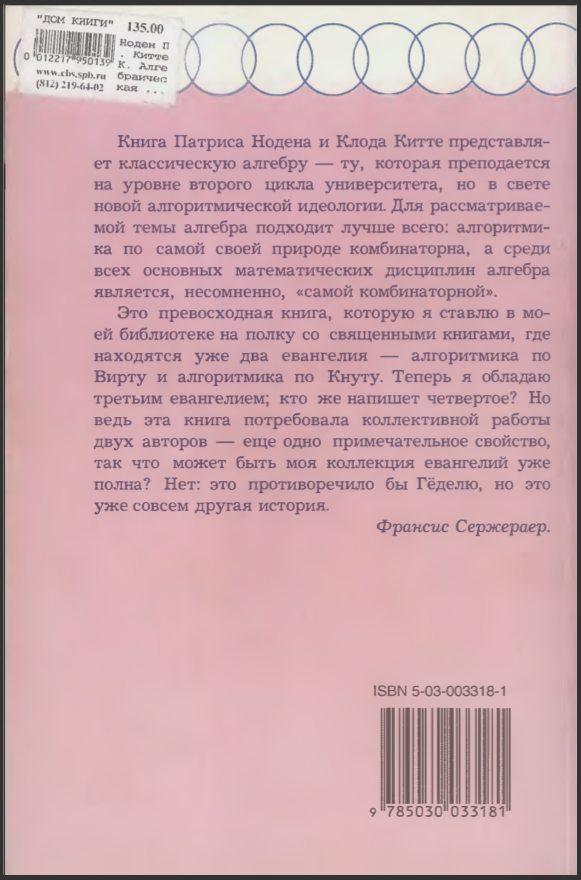
\includegraphics[width=1\linewidth]{NewVer}}
	\label{ris:image}
\end{figure}

%\newpage
%\thispagestyle{empty}
%\begin{figure}[ph]
%	\center{\includegraphics[width=1\linewidth]{MyVar}}
%	\label{ris:image}
%\end{figure}

\newpage

\end{document} 
